%!TEX root = parita-msc.tex

\chapter{\ac{owl} Ontology for Survey}
\label{chap:ontology}
\begin{doublespace}
\section{Development Tool for the Creation of New \ac{owl} Vocabularies}
\par In data science, for a fresh and developing branch like ontology engineering, it is difficult to find enough knowledge that can be reused. The field is still growing with research and development in progress as well as a lot still required to be explored in the future. As a result of this, linked open vocabularies are limited currently, and hence, the data publishers will have to create a vocabulary in case they do not find the required vocabulary from the already existing vocabularies.
\par There are editors available today that help the publishers to create their own linked open vocabularies. Alatrish at the University of Belgrad~\cite{alatrish2013comparison}, in 2013, compared the most used ontology editors, namely, Apollo, OntoStudio, Protégé, Swoop, and TopBraid Composer. The editors were compared based on the following features:
\begin{itemize}
  \item General description: developers' details, and accessibility on the internet (open source or software licensed)
  \item Software architecture and tools evaluation: semantic web architecture, support for plug-ins, backup management, and ontology storage
  \item Interoperability: interoperability with other ontology tools, support and translation for other languages
  \item Knowledge representation: Knowledge Representation (KR) paradigm of knowledge model, axiom language, and methodological support
  \item Inference services: built-in inference engine, other attached inference engines, and constraint/consistency checking
  \item Usability: graphical taxonomy, graphical views, zooms, collaborative working, and ontology libraries
\end{itemize}
\par After studying the details and comparison among the most used editors based on the above features by Alatrish~\cite{alatrish2013comparison}, Protégé has been used for the development of the instrument to support this research and thesis work.
\section{Protégé}
\par Stanford University developed a free, open-source ontology development platform, Protégé\footnote{https://protege.stanford.edu}, that offers a set of substantial tools\footnote{along with various plug-ins and Java-based \ac{api}} to build ontologies for knowledge-based applications and to implement various \say{knowledge-modeling structures and actions that support the creation, visualization and manipulation of ontologies in various representation formats}~\cite{alatrish2013comparison}. Protégé offers customization options to build knowledge models and to add data. 
\subsection{Usability of Protégé}
\par The \ac{iso} standard 9241\footnote{https://www.iso.org/standard/63500.html} defines usability as \say{the extent to which a product can be used by specified users to achieve specified goals with effectiveness, efficiency, and satisfaction in a specified context of use}. In usability engineering, Jacob Neilson~\cite{neilson1994usability} suggested five qualities of a usable product: \say{learnability, efficiency, memorability, errors (low rate,
easy to recover), and satisfaction}. These were the original five dimensions of usability which were then re-termed as all five words starting with \say{E} by Quesenbery~\cite{quesenbery2003dimensions}, and they became popular as the five Es of usability~\cite{quesenbery2003dimensions}. The new terms are as shown in Figure~\ref{fig:4.1}.
\begin{figure}[htp]
    \centering
    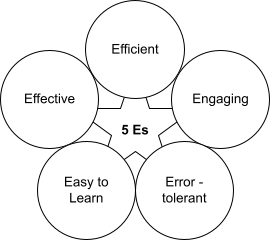
\includegraphics[width=12cm]{images/ch4/Figure1.png}
    \caption{Five Es of Usability}
    \label{fig:4.1}
\end{figure}
\begin{itemize}
  \item Effective: The task is completed accurately
  \par The user must be able to complete the desired task accurately using the design. If the user is unable to complete the task, irrespective of the time spent and efforts made to complete the task, the design is said to have failed to reach meet the design's goals. To measure effectiveness in a design, it is necessary to know users' perspectives of success and accuracy.
  \item Efficient: The task is completed quickly
  \par The user must be able to complete the task easily. The interface should be designed to allow the users to complete the desired tasks with the least complexity and within the minimum possible time. If a simple task takes more than the required time for completion, the design is not feasible and would be said to not meet the goals.
  \item Engaging: The look and feel of the design is interactive and engaging
  \par The look and feel of the interface must be interactive so that the user finds it interesting and continues using it. The user of the interface should be able to connect with the presentation and the organization of the components of the interface and hence should be satisfied by using the design to complete the desired task.
  \item Error-tolerant: Error prevention and data recovery in case any error is committed
  \par The interface should be able to easily handle errors. This means in case the user commits mistakes, the interface should be helpful enough to not lose the work done by the user along with providing the error correction options.
  \item Easy to learn: The interface should be easy to learn
  \par The user should get the feeling of familiarity and adaption while using the interface. The names of the components and tools in the design must be appropriate so that the user can understand their purpose from the name itself. For instance, in a banking application, using the keyword \say{balance owed} to denote the debit amount might confuse the user by not giving a clear idea about who owes the money, that is, whether the customer owes the amount to the bank or vice versa.
\end{itemize}
\par The five dimensions of usability can be considered while designing as well as for evaluation. While designing, the engineers consider the five dimensions as goals to be achieved whereas while testing and evaluation, they are considered as the requirements necessary for the designed model. The five dimensions of usability were used to assess the usability of Protégé and the report of the evaluation is as follows:
\begin{itemize}
  \item Effective: Protégé is an effective design as it allows the users to build ontologies and use other tools precisely. The users can complete the desired tasks accurately using the set of facilities available.
  \item Efficient: It is easy and straightforward to describe the vocabularies and build ontologies. All the desired tasks in Protégé can be completed quickly (without wasting much time) as it is easy to look for the facilities using the menus and tools available. Hence, Protégé is an efficient ontology builder.
  \item Engaging: The tools and menus in Protégé are interactive which leads to a better experience for the user. Also, the layout and the components are attractive and decent for the user to use this ontology builder whenever necessary. Overall, Protégé gives an engaging and satisfactory user experience.
  \item Error-tolerant: Protégé provides options for modifications, additions, and deletions of classes, objects, and properties, which allow the users to correct the errors that were committed. Also, the deleted classes can be recovered using \say{Undo} from the edit menu resulting in proving Protégé as an error-tolerant design.
  \item Easy to learn: Protégé is easy to learn as it has a familiar look and commonly used names for the tools and menus making it easy for the users to adapt and know them nicely. Also, the \say{Help} document along with a list of some frequently asked questions is available which helps the users in the correct direction whenever they are lost.
\end{itemize}
\section{Procedure to Model the Survey Ontology in \ac{owl} Using Protégé Tools}
\par This section focuses on a step-wise methodology that has been followed to create new \ac{owl} vocabularies for a survey using Protégé. Figure~\ref{fig:4.2} shows the student feedback form for which the new vocabularies are described. Protégé is available for use as a web application. Protégé can also be downloaded\footnote{https://protege.stanford.edu/products.php\#desktop-protege} to use as a desktop application for ontology construction and visualization.
\begin{figure}[htp]
    \centering
    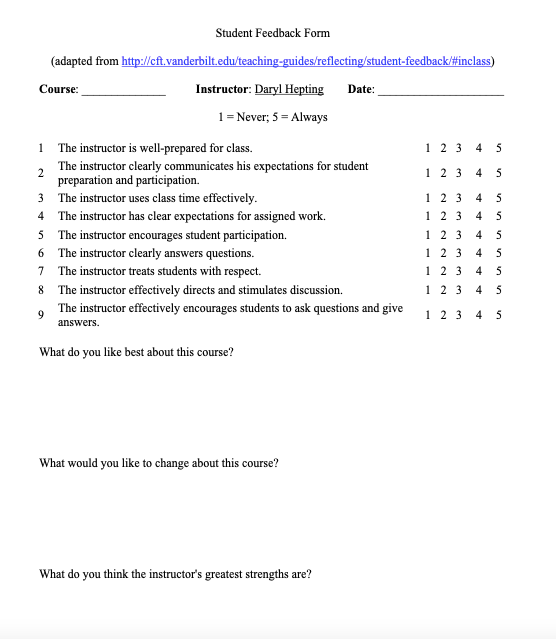
\includegraphics[width=15cm]{images/ch4/Figure2.png}
    \caption{The Student Feedback Form, from Hepting~\cite{prof}}
    \label{fig:4.2}
\end{figure}
\par To commence with the process of building the survey ontology, a new project needs to be created with a unique \ac{iri}\footnote{https://www.w3.org/2011/rdf-wg/wiki/IRIs/RDFConceptsProposal}  and the ontology version. Figure~\ref{fig:4.3} shows the Protégé home-screen with a new project created and an \ac{iri} with the name and version of ontology.
\begin{figure}[htp]
    \centering
    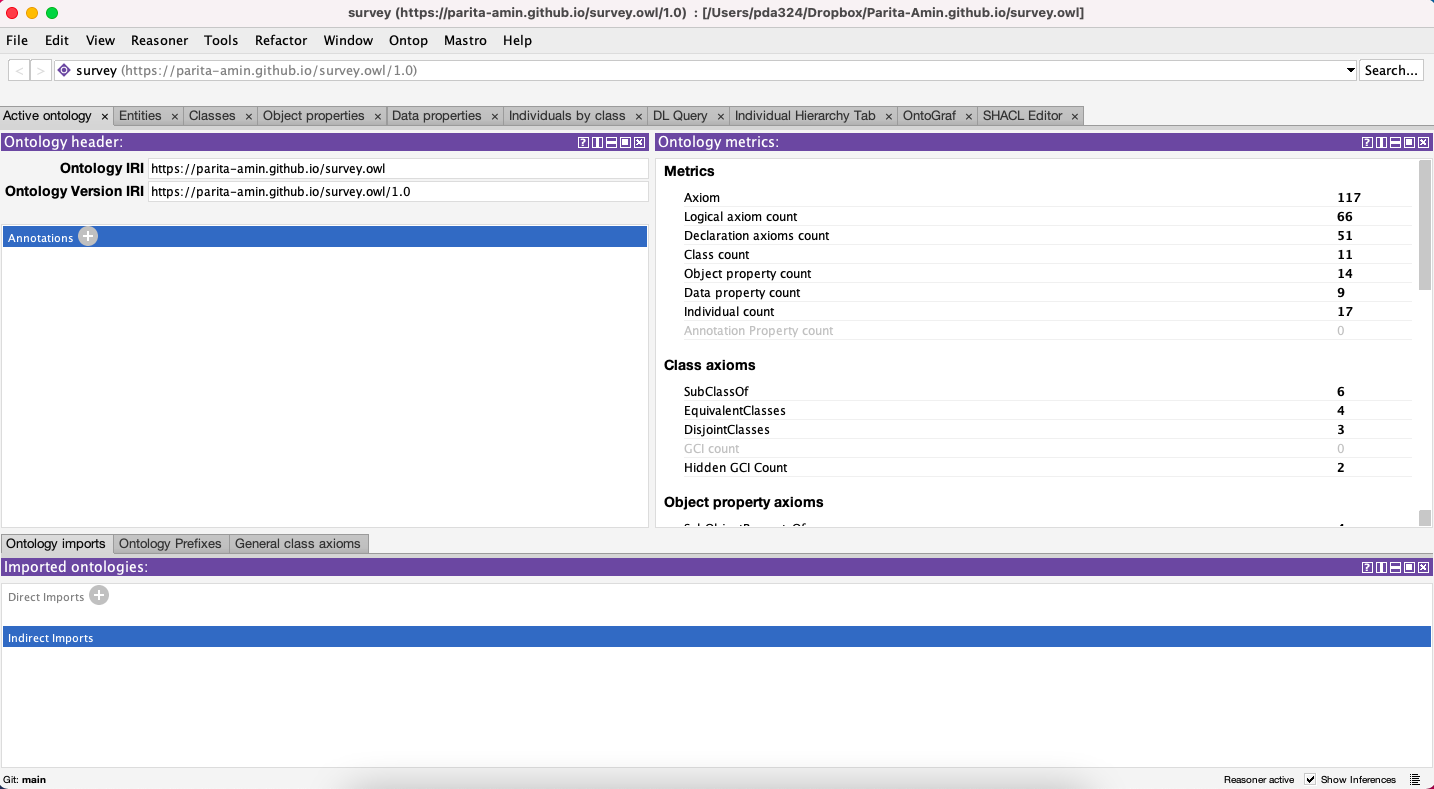
\includegraphics[width=15cm]{images/ch4/Figure3.png}
    \caption{Protégé Home-screen for a New Project with an Ontology Name and an IRI}
    \label{fig:4.3}
\end{figure}
\subsection{Classes and Class Hierarchy}
\par The next step is to create classes and build the hierarchy for the class nodes. Each entity in Protégé is directly or indirectly a child node of the \say{Thing} class. Also, each object has a name-value pair, which generally are the nodes of the \say{Domain\_Entity} class, an inherited class of Thing. Initially, four classes, \say{Thing}, \say{Domain\_Entity}, \say{Independent\_Entity}, and \say{Value} are created using class hierarchy, as shown in Figure~\ref{fig:4.4}. To create a class hierarchy for the classes that represent entities in the survey, there are three steps to be followed:
\begin{figure}[htp]
    \centering
    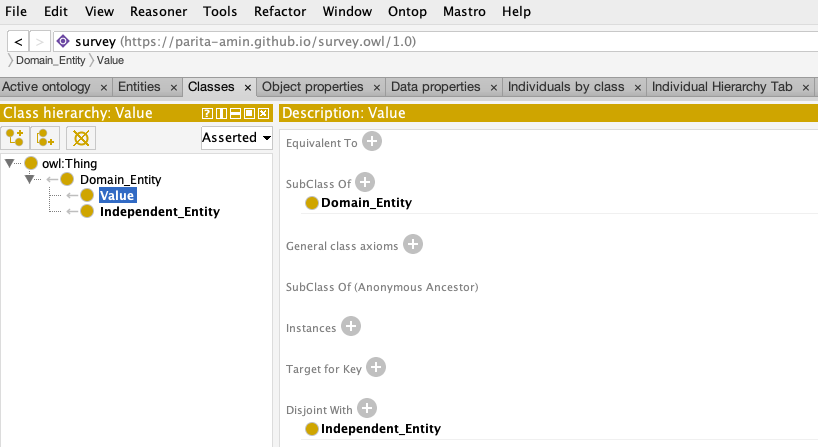
\includegraphics[width=15cm]{images/ch4/Figure4.png}
    \caption{Class Hierarchy of Thing, Domain\_Entity, Independent\_Entity, and Value}
    \label{fig:4.4}
\end{figure}
\begin{enumerate}
    \item Select \say{owl:Thing} in the Class Hierarchy View of the Classes tab from the Windows menu followed by selecting \say{Create class hierarchy...} from the Tools menu, as shown in Figure~\ref{fig:4.5} to open a \say{Enter hierarchy} pop-up window which allows the users to add classes to the ontology.
    \begin{figure}[htp]
    \centering
    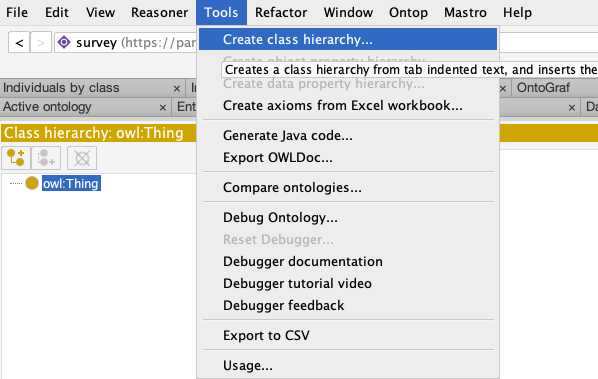
\includegraphics[width=15cm]{images/ch4/Figure5.png}
    \caption{Tools Menu to Create Class Hierarchy}
    \label{fig:4.5}
\end{figure}
    \item Enter the class names in the pop-up window starting from the left. For the child nodes, leave some spaces before writing the class name. Each horizontal line consists of one class name, as shown in Figure~\ref{fig:4.6}. 
    \begin{figure}[htp]
    \centering
    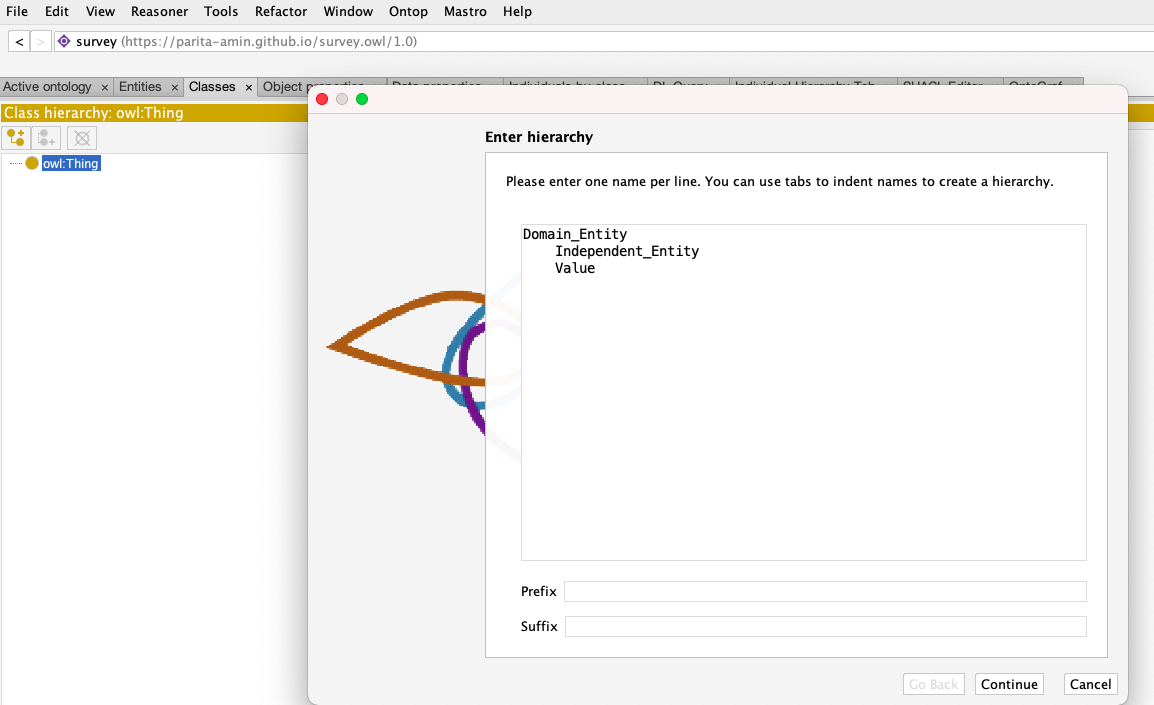
\includegraphics[width=15cm]{images/ch4/Figure6.png}
    \caption{\enquote{Enter hierarchy} Pop-up Window}
    \label{fig:4.6}
\end{figure}
    \item On clicking \say{Continue} on the pop-up window in Figure~\ref{fig:4.6}, it opens up a new pop-up window. Here, it is important to state whether one wants the sibling classes to be disjoint or not. The checkbox needs to be checked accordingly. Usually, it is recommended to create disjoint sibling classes which can be changed later as necessary, as shown in Figure~\ref{fig:4.7}.
    \begin{figure}[htp]
    \centering
    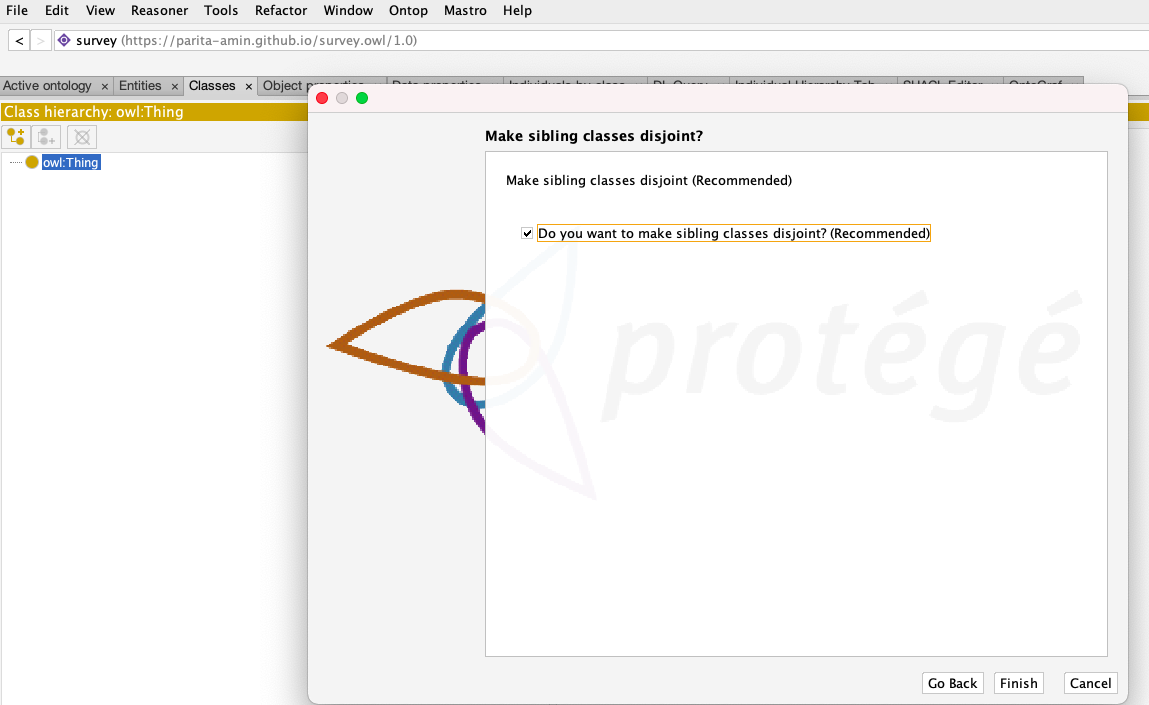
\includegraphics[width=15cm]{images/ch4/Figure7.png}
    \caption{Pop-up Window to Create Disjoint Sibling Classes}
    \label{fig:4.7}
\end{figure}
\end{enumerate}
\par Once the classes are added, the next step is to describe the classes. Descriptions of classes like \say{Equivalent to}, \say{SubClass Of}, \say{Instances}, \say{Disjoint With} and so on can be added using the Description view of the Class tab (shown in Figure~\ref{fig:4.4}). Each class can be described individually by selecting a particular class and adding details to the description view. 
\par All the classes can be created and described using the above steps. In the end, the class hierarchy for the survey ontology would be as shown in Figure~\ref{fig:4.8}. The survey can have \say{Respondent}, \say{Response Date}, \say{Type of Survey}, \say{Survey Questions}, \say{Survey Answers}, and \say{Likert Scale}, which are considered for this ontology as well. Here, the type of survey used is \say{feedback survey}. The survey questions and survey answers would further have entities corresponding to various forms of question-answer. Generally, feedback surveys consist of two types of questions, namely, \say{Likert Questions} and \say{Open-ended Questions}. The type of questions might differ depending on the designer of the survey, some of which, as stated on the \emph{SurveyMonkey}\footnote{https://www.surveymonkey.com/mp/survey-question-types/} website, are listed below. 
\begin{figure}[htp]
    \centering
    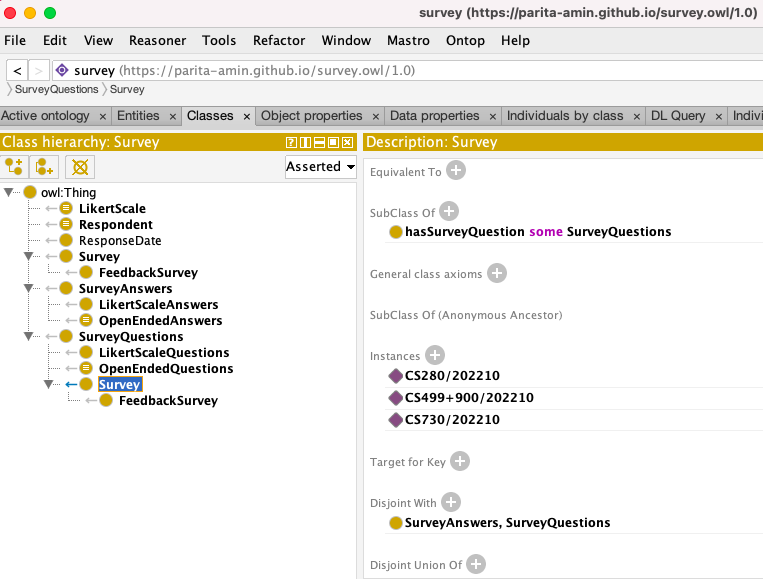
\includegraphics[width=15cm]{images/ch4/Figure8.png}
    \caption{Class Hierarchy in Survey Ontology}
    \label{fig:4.8}
\end{figure}
\begin{multicols}{2}
\begin{itemize}
    \item Multiple Choice Questions
    \item Rating Scale Questions
    \item Likert Scale Questions
    \item Matrix Questions
    \item Dropdown Questions
    \item Open-ended Questions
    \item Demographic Questions
    \item Ranking Questions
    \item Image Choice Questions
    \item Click Map Questions
    \item File Upload Questions
    \item Slider Questions
    \item Benchmarkable Questions
\end{itemize}
\end{multicols}
\par For this research, the feedback survey that has been considered has Likert and Open-ended questions. The entities described for the questions and answers are \say{LikertScaleQuestions}, and \say{OpenEndedQuestions} as sub-classes of \say{SurveyQuestions}, and \say{LikertScaleAnswers}, and \say{OpenEndedAnswers} as sub-classes of \say{SurveyAnswers}.
\par For all the survey questions, there would be a question and an answer, where both of them would be considered as distinct entities. Likert questions are the questions for which the answers are from the preset list of answers. For the Likert questions, the questions can be either of type \say{Never-Always-4} or \say{Never-Always-5} or \say{Never-Always-7} or \say{Never-Always-*}, of which Never-Always-5 has been used by Hepting~\cite{prof}. In a Never-Always-5 type of survey, 5 degrees of agreement are used as shown in Table~\ref{table:4.1}. In addition to these degrees, this ontology also considers the instances where the question wouldn't be answered. In this case, the field corresponding to the answer is left blank. On the other hand, Open-ended questions have unpredictable answers and hence there cannot be any degree of measurement for Open-ended questions.
\begin{table}[h!]
    \centering
    \begin{tabular}{|c|l|}
    \hline Number \ & Agreement \\ \hline
     1 & Never\\ \hline
     2 & [Rarely]\\ \hline
     3 & [Sometimes]\\ \hline
     4 & [Often]\\ \hline
     5 & Always\\ \hline
    \end{tabular}
    \caption{Degrees of Agreement for Likert-scale Questions}
    \label{table:4.1}
\end{table}
\subsection{Object Properties and Object Property Hierarchy}
\par The next step in building the ontology, after describing the classes, is describing the \say{Object Properties}. Object properties are used to link the entities (classes in Protégé). The \say{owl:topObjectProperty} is the root node of the object properties' hierarchy. The hierarchy for object properties can be built by selecting a property in the Object Property Hierarchy view of the Object Property Views tab and then going to the tools menu as shown in Figure~\ref{fig:4.9}. The remaining steps are similar to the ones that are followed for building class hierarchy (Figure~\ref{fig:4.5}, ~\ref{fig:4.6}, and ~\ref{fig:4.7}).
\begin{figure}[htp]
    \centering
    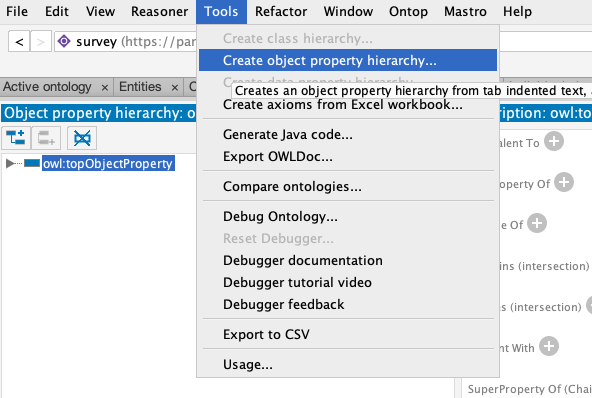
\includegraphics[width=15cm]{images/ch4/Figure9.png}
    \caption{Tools Menu to Create Object Property Hierarchy}
    \label{fig:4.9}
\end{figure}
\par Also, the description view of object properties hierarchy allows the user to describe the object properties. The details that can be added or modified using the description view are \say{Equivalent To}, \say{SubProperty Of}, \say{Inverse Of}, \say{Domains (intersection)}, \say{Ranges (intersection)}, \say{Disjoint With}, and \say{SuperProperty Of (Chain)}. 
\par The names of the object properties usually start with an \say{is} or a \say{has}. For instance, consider two classes: \say{Lady} (class 1) and \say{Parita} (class 2). To describe the link between class 1 (Lady) and class 2 (Parita) such that class 1 has value class 2 and class 2 is value of class 1, the properties \say{hasName} and \say{isNameOf} would be used respectively, as shown in Figure~\ref{fig:4.10}. 
\begin{figure}[htp]
    \centering
    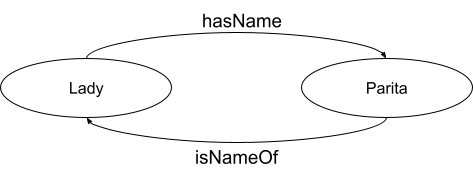
\includegraphics[width=15cm]{images/ch4/Figure10.png}
    \caption{Object Properties for Classes \enquote{Lady} and \enquote{Parita}}
    \label{fig:4.10}
\end{figure}
\par Each object property might have a corresponding inverse property. For the above instance, it can be said that:
\begin{center}
    \par Lady hasName Parita \textbf{is equivalent to} Parita isNameOf Lady
\end{center}
Here, \say{hasName} is inverse of \say{isNameOf} and \say{isNameOf} is inverse of \say{hasName}. Apart from inverse, domain and range\footnote{http://protegeproject.github.io/protege/views/object-property-description/} are two other important parts of description of object properties. According to Horridge et al.~\cite{horridge2009practical}, in \ac{owl}, \say{domain and range are not constraints to be checked. They are axioms which are used by the reasoner to make inferences}. As shown in Figure~\ref{fig:4.11}, \say{Lady} acts as the \say{Domain} and \say{Parita} acts as the \say{Range} for \say{hasName} whereas for \say{isNameOf}, \say{Parita} is the \say{Domain} and \say{Lady} is the \say{Range}. 
\begin{figure}[htp]
    \centering
    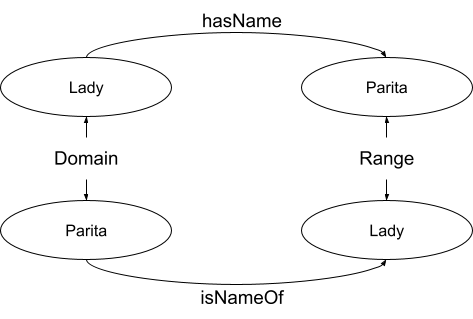
\includegraphics[width=12cm]{images/ch4/Figure11.png}
    \caption{Domain and Range Classes for \enquote{hasName} and \enquote{isNameOf}}
    \label{fig:4.11}
\end{figure}
\par Using the above method of naming and building object properties, some of the primary object properties are described for the survey ontology as shown in Figure~\ref{fig:4.12} where as Table~\ref{table:4.2} shows the list of the object properties along with their domain and range classes (entities). Table~\ref{table:4.3} consists of the parent nodes and inverse properties of the object properties. The three parent nodes involved in object property hierarchy are \say{owl:TopObjectProperty}, \say{hasContent}, and \say{isContentOf}. Protégé has a built-in \say{Reasoner} that allows the users to determine inconsistencies of a class as well as to discover implicit information.
\begin{figure}[htp]
    \centering
    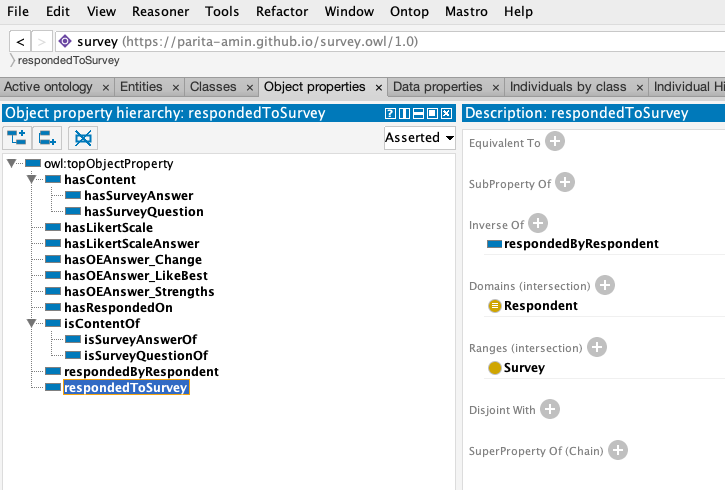
\includegraphics[width=15cm]{images/ch4/Figure12.png}
    \caption{Object Property Hierarchies, Domain and Range for Classes}
    \label{fig:4.12}
\end{figure}
\begin{table}[h!]
    \centering
    \begin{tabular}{|l|l|l|} 
    \hline Object Property & Domain & Range\\ \hline
     hasSurveyQuestion & Survey & SurveyQuestions\\ \hline
     hasLikertScale & LikertScaleQuestions & LikertScale\\ \hline
     hasLikertScaleAnswer & Respondent & LikertScale\\ \hline
     hasRespondedOn & Respondent & ResponseDate\\ \hline
     respondedToSurvey & Respondent & Survey\\ \hline
     hasOEAnswer\_Change & OpenEndedQuestions & OpenEndedAnswers\\ \hline
     hasOEAnswer\_LikeBest & OpenEndedQuestions & OpenEndedAnswers\\ \hline
     hasOEAnswer\_Strengths & OpenEndedQuestions & OpenEndedAnswers\\ \hline
    \end{tabular}
    \caption{Object Properties and Their Domain and Range}
    \label{table:4.2}
    \end{table}
\begin{table}[h!]
    \centering
    \begin{tabular}{|l|l|l|} 
    \hline Object Property & Parent Node & Inverse Property\\ \hline
     hasContent & owl:TopObjectProperty & isContentOf\\ \hline
     isContentOf & owl:TopObjectProperty & hasContent\\ \hline
     hasLikertScale & owl:TopObjectProperty & \\ \hline
     hasLikertScaleAnswer & owl:TopObjectProperty & \\ \hline
     hasOEAnswer\_Change & owl:TopObjectProperty & \\ \hline
     hasOEAnswer\_LikeBest & owl:TopObjectProperty & \\ \hline
     hasOEAnswer\_Strengths & owl:TopObjectProperty & \\ \hline
     hasRespondedOn & owl:TopObjectProperty & \\ \hline
     respondedByRespondent & owl:TopObjectProperty & respondedToSurvey\\ \hline
     respondedToSurvey & owl:TopObjectProperty & respondedByRespondent\\ \hline
     hasSurveyQuestion & hasContent & isSurveyQuestionOf\\ \hline
     hasSurveyAnswer & hasContent & isSurveyAnswerOf\\ \hline
     isSurveyQuestionOf & isContentOf & hasSurveyQuestion\\ \hline
     isSurveyAnswerOf & isContentOf & hasSurveyAnswer\\ \hline
    \end{tabular}
    \caption{Object Properties with Their Parent Nodes and Inverse Properties}
    \label{table:4.3}
    \end{table}
\subsection{Data Properties and Data Property Hierarchy}
\par Furthermore, the \say{Data Properties} can also be described for ontology. \say{An ontology data property provides a relation to attach an entity instance to some literal datatype value (an \ac{rdf} number, string or data for example) that is a measure or estimate of what that data property is about.}\footnote{https://ddooley.github.io/docs/data-properties/} In Protégé, the \say{owl:topDataProperty} is the root node of the data properties' hierarchy. The data property hierarchy can be built by selecting a property in the Data Property Hierarchy view of the Data Property Views tab and then going to the tools menu as shown in Figure~\ref{fig:4.13}. The remaining steps are similar to the ones that are followed for building class and object property hierarchy (Figure~\ref{fig:4.5}, ~\ref{fig:4.6}, and ~\ref{fig:4.7}). 
\begin{figure}[htp]
    \centering
    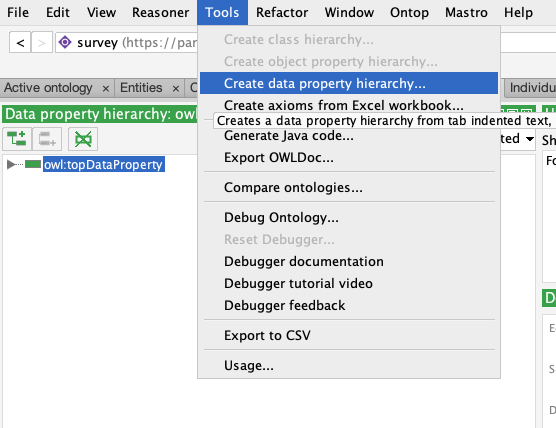
\includegraphics[width=15cm]{images/ch4/Figure13.png}
    \caption{Tools Menu to Create Data Property Hierarchy}
    \label{fig:4.13}
\end{figure}
\par Data properties can be described using the description view of data properties of hierarchy which included details like \say{Equivalent To}, \say{SubProperty Of}, \say{Domains (intersection)}, \say{Ranges}, and  \say{Disjoint With}. Figure~\ref{fig:4.14} shows the data properties described for the survey ontology. The parent node of all the data properties is \say{owl:topDataProperty} and the domain and range for all the data properties are \say{Respondent} and \say{xsd:positiveInteger} respectively. Table~\ref{table:4.4} consists of list of data properties along with their domain and range classes (entities).
\begin{figure}[htp]
    \centering
    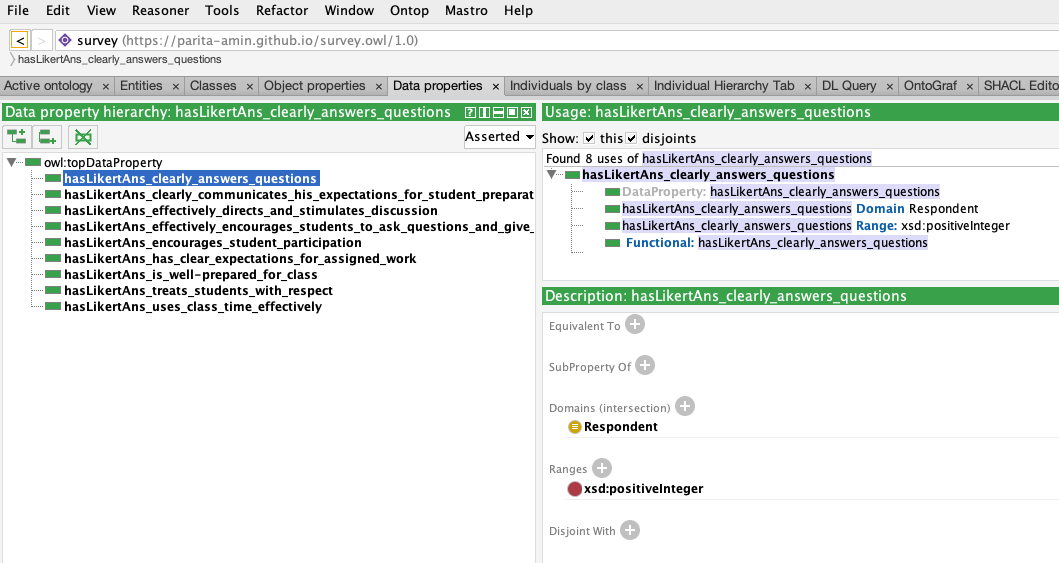
\includegraphics[width=15cm]{images/ch4/Figure14.png}
    \caption{Data Property Hierarchies, Domain and Range for Classes}
    \label{fig:4.14}
\end{figure}
\begin{table}[h!]
    \centering
    \begin{tabular}{|l|l|l|} 
    \hline \ \ \ \ \ \ \ \ \ \ \ \ \ \ \ Data Property &\ Domain &\ \ \ \ \ \ \ Range\\ \hline
     hasLikertAns\_is\_well-prepared\_for&\\ \_class & \multirow{-2}{5em}{Respondent} & \multirow{-2}{8.5em}{xsd:positiveInteger}\\ \hline
     hasLikertAns\_clearly\_communicates&\\ \_his\_expectations\_for\_student&\\ \_preparation\_and\_participation & \multirow{-3}{5em}{Respondent} & \multirow{-3}{8.5em}{xsd:positiveInteger}\\ \hline
     hasLikertAns\_uses\_class\_time&\\ \_effectively & \multirow{-2}{5em}{Respondent} & \multirow{-2}{8.5em}{xsd:positiveInteger}\\ \hline
     hasLikertAns\_has\_clear\_expectations&\\ \_for\_assigned\_work & \multirow{-2}{5em}{Respondent} & \multirow{-2}{8.5em}{xsd:positiveInteger}\\ \hline
     hasLikertAns\_encourages\_student&\\ \_participation & \multirow{-2}{5em}{Respondent} & \multirow{-2}{8.5em}{xsd:positiveInteger}\\ \hline
     hasLikertAns\_clearly\_answers&\\ \_questions & \multirow{-2}{5em}{Respondent} & \multirow{-2}{8.5em}{xsd:positiveInteger}\\ \hline
     hasLikertAns\_treats\_students&\\ \_with\_respect & \multirow{-2}{5em}{Respondent} & \multirow{-2}{8.5em}{xsd:positiveInteger}\\ \hline
     hasLikertAns\_effectively\_directs&\\ \_and\_stimulates\_discussion & \multirow{-2}{5em}{Respondent} & \multirow{-2}{8.5em}{xsd:positiveInteger}\\ \hline
     hasLikertAns\_effectively\_encourages&\\ \_students\_to\_ask\_questions\_and&\\ \_give\_answers & \multirow{-3}{5em}{Respondent} & \multirow{-3}{8.5em}{xsd:positiveInteger}\\ \hline
    \end{tabular}
    \caption{Data Properties and Their Domain and Range}
    \label{table:4.4}
    \end{table}
\subsection{Individuals}
\par 
\par After describing the classes, object properties, data properties, and individuals, the next step is to determine and fix the errors and inconsistencies in the ontology using a Reasoner. The final class hierarchy of the \ac{owl} ontology in Protégé, after using the HermiT 1.4.3.456 reasoner, would be as shown in Figure~\ref{fig:4.15}.
\begin{figure}[htp]
    \centering
    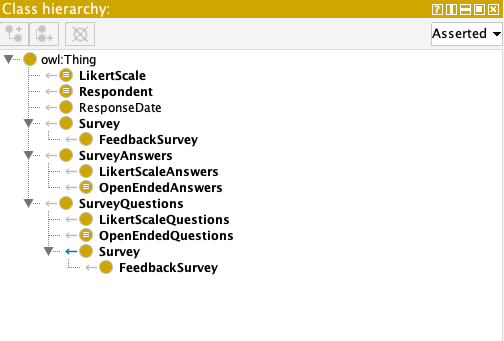
\includegraphics[width=15cm]{images/ch4/Figure15.png}
    \caption{Class Hierarchy for the Final Version of Survey Ontology}
    \label{fig:4.15}
\end{figure}
\par The grey (all entities) and blue (\say{Survey} entity) back arrows in front of the yellow solid dot, which indicates class, show parent/child relationship other than that of SubClassOf. This feature can be enabled and disabled by selecting \say{Display relationship in class hierarchy} option from the \say{View} menu of Protégé. Figure~\ref{fig:4.16} shows the relation indicated by the blue back arrow.
\begin{figure}[htp]
    \centering
    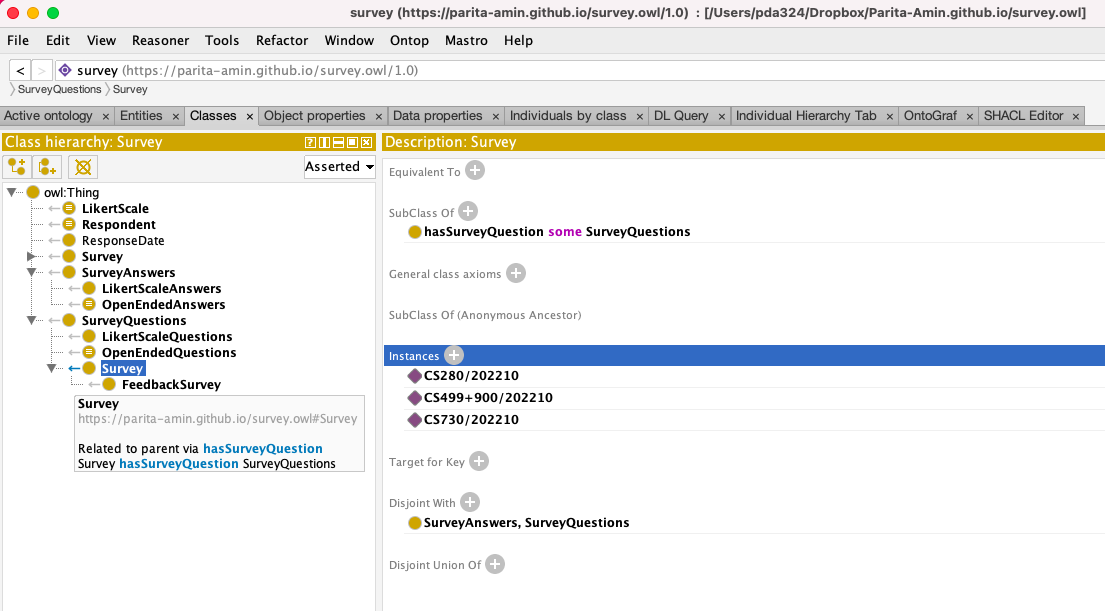
\includegraphics[width=15cm]{images/ch4/Figure16.png}
    \caption{Parent/Child Relation indicated by "Blue Back" Arrow}
    \label{fig:4.16}
\end{figure}
\section{Visualization Tools for \ac{owl} Ontology}
\par The next step is visualization of the built \ac{owl} ontology using various visualization tools. Protégé supports plug-ins for some visualization tools like OntoGraf and \ac{owl}Viz whereas tools like WebVOWL, RelFinder and \ac{owl}GrEd are available for use as web-based tools. This section focuses on the two tools, OntoGraf and WebVOWL, used for the visualization of the survey ontology in this research.
\subsection{OntoGraf}
\par Falconer~\cite{falconer2010ontograf} introduced OntoGraf as a Protégé plug-in for the visualization of the \ac{owl} ontologies. This tool helps the users to represent the ontologies, built using Protégé, by repetitively allowing and restricting the desired classes. OntoGraf offers various graph layout options for visualization like Grid Layout\footnote{classes are arranged in a grid alphabetically}, Spring Layout, and Tree Layout\footnote{both horizontal and vertical}. Antoniazzi and Viola~\cite{antoniazz2018rdf} stated that the \say{individuals of a class can be visualized in its tooltip, but this is uncomfortable when dealing with a high number of assertional statements}. The graphs generated using OntoGraf can be exported as image files of various formats such as \ac{png}, \ac{jpeg}, \ac{gif} and as a dot file\footnote{a Microsoft Word Template with the details of default settings}.
\par Figure~\ref{fig:4.17} shows the graph generated using OntoGraf for the survey ontology. To start with the graph formation, the classes \say{Thing}, \say{Domain\_entity}, \say{Independent\_entity} and \say{Value} were selected followed by expansion of \say{Independent\_entity} and \say{Value} classes by double-clicking them. This expansion adds all the classes that are connected to the classes. The classes connected includes both the subclasses as well as the ones linked through the object properties. Solid blue lines are used to denote the relationships between the classes and their subclasses whereas dashed lines are used to represent the object properties.
\begin{figure}[htp]
    \centering
    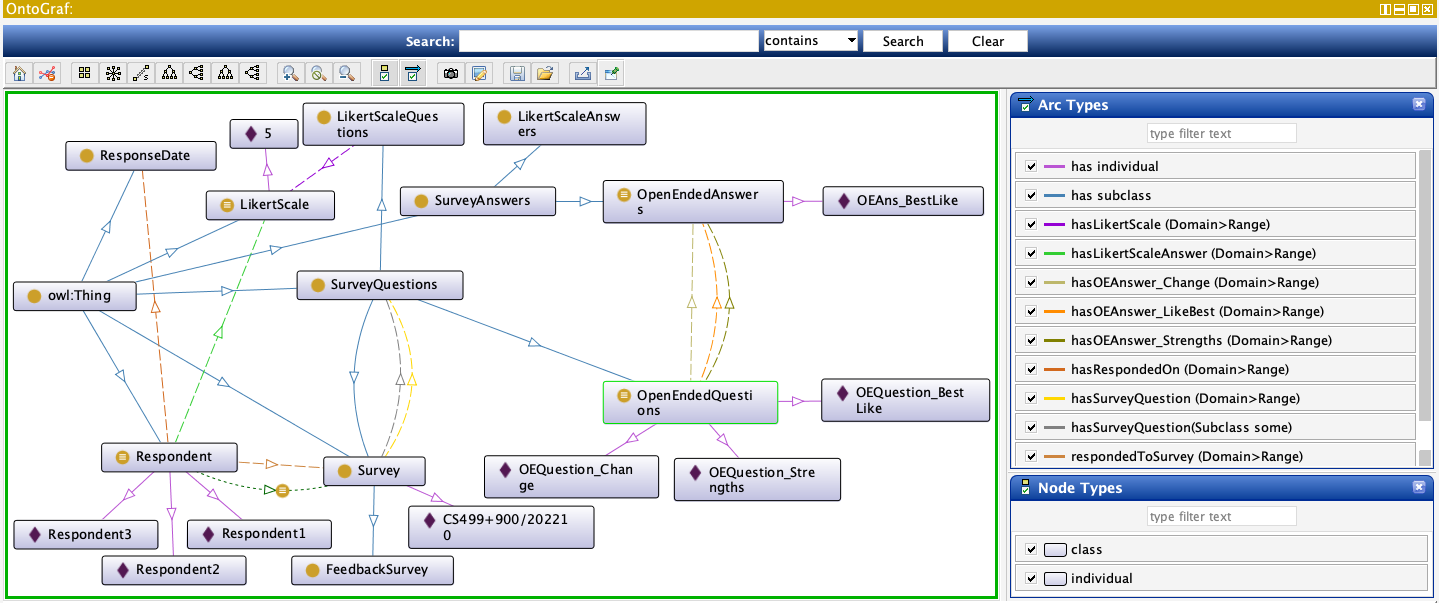
\includegraphics[width=15cm]{images/ch4/Figure17.png}
    \caption{OntoGraf for Survey Ontology}
    \label{fig:4.17}
\end{figure}
\subsection{WebVOWL}
\par WebVOWL~\cite{lohmann2014webvowl}, the Web-based \ac{vowl}, one of the variety of forms in which the \ac{vowl} visualization tool is available, represents the \say{ontologies graphically using a force-directed graph layout}~\cite{antoniazz2018rdf}. \ac{vowl} follows some ground rules for the representation of \ac{owl} ontologies which are:
\begin{enumerate}
    \item Circles are used to denote classes. Also, different types are assigned different colors. For instance, \ac{owl} classes are denoted using \say{light blue circles}.
    \item Black solid lines are used to represent \ac{owl} object and datatype properties. The object properties use light blue labels where as the datatype properties are labelled in green.
    \item The relationships between the classes and their subclasses are represented using dashed lines.
\end{enumerate}
\par Figure~\ref{fig:4.18} shows the graphical representation of the survey ontology using Web\ac{vowl}. The figure focuses on only some of the class-subclass relationships and some of the object properties. The metadata and the statistics of the node (circle) or the edge (line) can be retrieved by clicked on them. The entities (classes) and their relationships (object and datatype properties) can be presented or restricted using filters. The \ac{vowl} graph can be exported as an \ac{svg} image file or a \ac{json} code file.
\begin{figure}[htp]
    \centering
    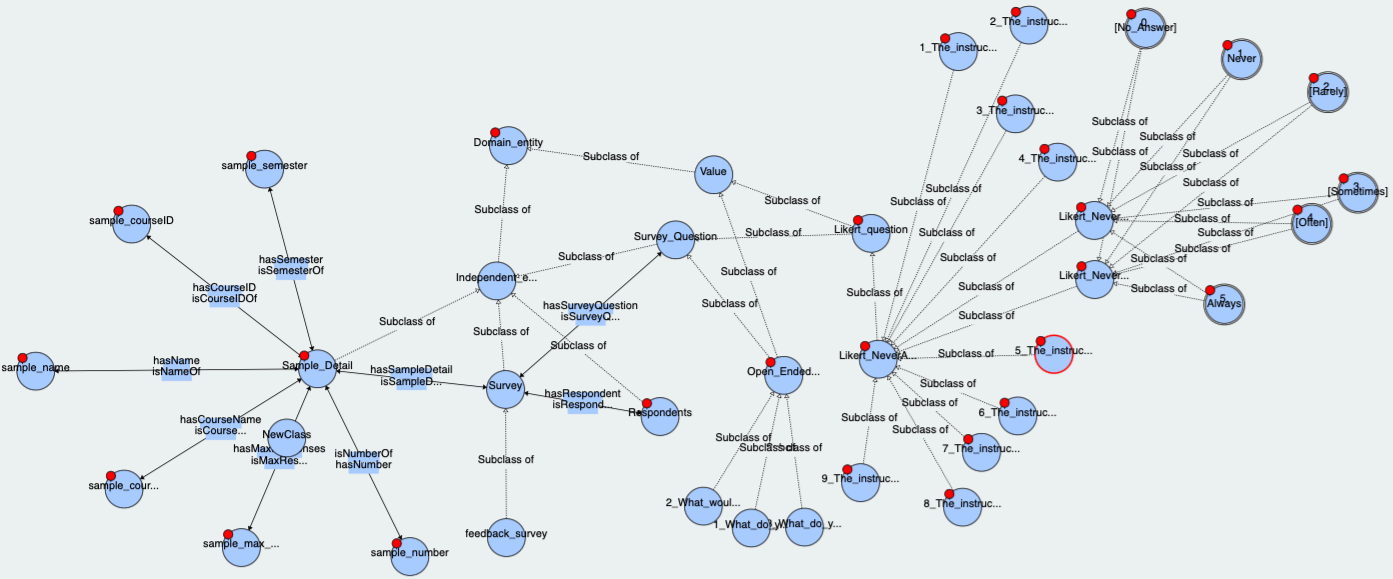
\includegraphics[width=15.5cm]{images/ch4/Figure18.png}
    \caption{WebVOWL for Survey Ontology}
    \label{fig:4.18}
\end{figure}
\end{doublespace}